\chapter{Profiles} 
\label{chapter:profiles}

\begin{center}

\includegraphics[scale=0.4]{../graphics/johnny_automatic_Jack_victorious.eps}
\end{center}

\lettrine{A}{lo largo de todo} este \pfc{} se han mencionado los \profiles{} en múltiples ocasiones y lo útiles que son o lo bien que encajan con el concepto de crear comunidades de práctica de una forma rápida y cómoda para un administrador o docente. Pero es aquí, en este capítulo, en el que se tratará de explicar de manera profunda qué son y cómo funcionan. Para lograrlo, se ha hecho una división del mismo en dos partes fundamentales: en la primera, veremos la teoría básica que sustenta los \profiles{}, primero a vista de pájaro, es decir, entenderemos el concepto y aprenderemos a manejar la herramienta en \tiki{} utilizando para ello un ejemplo real; en la segunda, se darán breves detalles técnicos de la implementación interna, es decir, del código fuente responsable del funcionamiento por si el lector desea modificar la herramienta a sus necesidades concretas. 

\section{¿Por qué surgen los Profiles?}

\tiki{}, al ser un \textit{software} muy completo, posee muchas características implementadas en su interior. Como usuarios de la plataforma podemos tomar ventaja de dicha arquitectura para construir casi cualquier cosa que deseemos. Pero, por norma general, resulta que muchas veces no queremos utilizar todas las herramientas que tenemos disponibles para implementar todos los posibles casos de uso que existen, si no que, dependiendo de nuestras necesidades específicas, modificamos la plataforma para realizar algo en concreto (utilizamos un subconjunto de ella). Por ejemplo: podríamos querer usar \tiki{} como un sistema para administrar nuestro \textit{blog}, o para hacer una \textit{wiki} corporativa para uso interno de la empresa en la que trabajamos, o para crear un foro de una comunidad de amantes del motor\ldots{} Como ya se ha comentado anteriormente, somos nosotros quienes ponemos límites a lo que queremos realizar.

Pero, uno de los problemas que ha arrastrado \tiki{} desde sus primeras versiones y hasta hace bien poco es que, con todas las características que posee la plataforma, ¿cuál es la mejor forma de estructurar los paneles de administración de una manera eficiente y que promueva la facilidad de uso entre sus usuarios? La respuesta a esta pregunta es que los desarrolladores de \tiki{} todavía no lo han conseguido (si, incluso hasta en las versiones más modernas siguen adoleciendo de este problema). A lo largo de la vida del proyecto han modificado, en varias ocasiones, los paneles de administración para hacerlos más intuitivos, pero, 1500 opciones de configuración posibles son demasiadas opciones a tener en cuenta. Esto hace que cualquier usuario que quiera manejar la plataforma tenga que dedicar una considerable cantidad de tiempo en aprender las entrañas del programa. Además otro problema, análogo al anterior, es que no sólo existen los paneles de administración principales (como los que vimos en el \chapterref{conceptos-fundamentales-tiki}), si no que también hay otros paneles secundarios (también dedicados para propósitos administrativos) que están distribuidos por diferentes partes de la plataforma.

Debido a los inconvenientes expuestos, a partir de la versión 4 de \tiki{}, se decidió hacer una reescritura masiva de todas las librerías principales y se comenzó a trabajar con el proyecto de los \profiles{}. A día de hoy, y en la versión 8, todavía continúan integrando y mejorando esta herramienta. Lo que está claro es que es una parte importante de la plataforma y así lo seguirá siendo en los próximos años, ya que, los \profiles{} solucionan el problema conocido como: \textit{la paradoja de la elección}\footnote{Esta teoría fue propuesta por Barry Schwartz en su libro \work{The Paradox of Choice: Why More Is Less} donde plantea que el exceso de opciones nos lleva a la parálisis y a la inacción. Y el problema posterior que surge: ansiedad, cuando hemos elegido \cite{libro:la-paradoja-de-la-elección}.}.

\section{¿Qué son los Profiles?}

Un \textit{Profile} no es más que un archivo de texto (que se encuentra almacenado en una página \textit{wiki} normal y corriente) con una serie de instrucciones que explican, paso a paso, que deseamos modificar de cualquiera de las 1500 preferencias de \tiki{}, permitiéndonos también, el poder crear, cambiar y borrar cualquier recurso que queramos. Para ello, hay una herramienta dentro de la librería de los \profiles{} encargada de traducir el texto contenido en una página \textit{wiki} en acciones concretas de la plataforma (\figureref{flujo_accion_profile}).

\begin{figure}[h!]
\centering
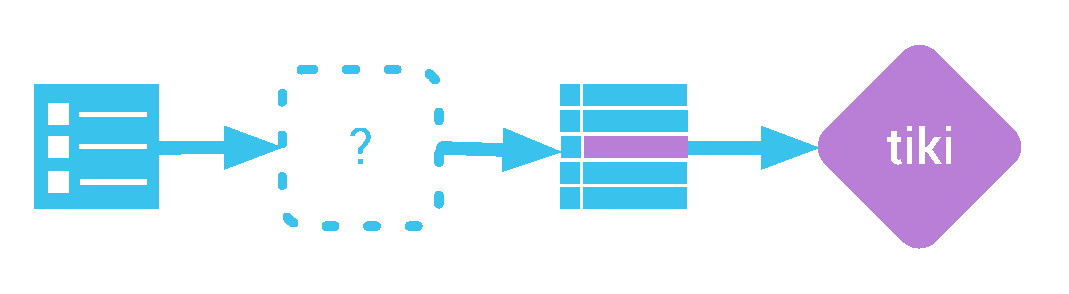
\includegraphics[width=\linewidth]{../graphics/fig_flujo_accion_profile.eps}
\caption{Un \profile{} \textit{modifica} las preferencias de \tiki{} de la manera en la que esté especificado. El rectángulo con el interrogante es el traductor que se encarga de \q{entender} lo que el \profile{} desea alterar (veremos más detalles internos en la \sectionref{componentes-profiles}).}\label{fig:flujo_accion_profile}
\end{figure}

Si recordamos nuestro periplo por el \chapterref{conceptos-fundamentales-tiki}, buena parte de éste se dedicó a explicar muchos conceptos \textit{críticos} de \tiki{} a la vez que se demostraban cuales eran los pasos que tenía que seguir un administrador para poder crear \textit{una} comunidad de práctica.
En lugar de tener que lidiar con los paneles de administración, una opción es que podemos concebir un \profile{} que explique, como si de una receta de cocina se tratase, como se debe crear una comunidad de práctica (\figureref{etapas_profile}). (Y De esta manera podemos automatizar un proceso que es de índole repetitiva.)

\begin{figure}[h!]
\centering
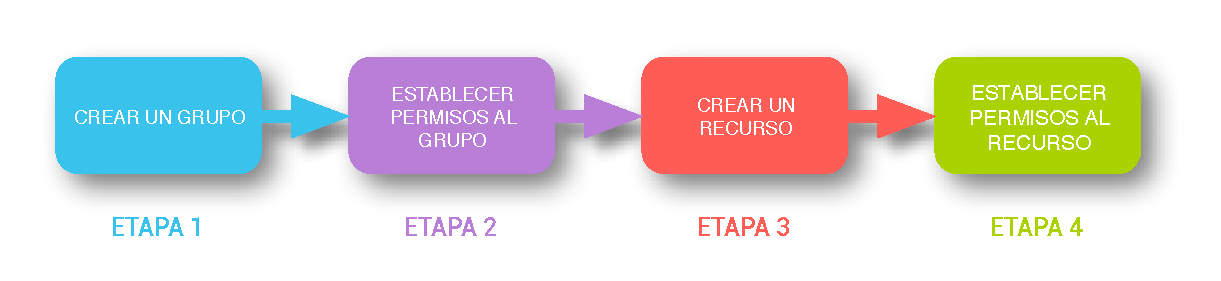
\includegraphics[width=\linewidth]{../graphics/fig_etapas_profile.eps}
\caption{Para cada \profile{} hay que definir exactamente que deseamos ejecutar. Una forma de crear un \profile{} con éxito es dividir lo que queremos crear en etapas.}\label{fig:etapas_profile}
\end{figure}

La parte buena del asunto es que, con los \profiles{}, al ser realmente páginas \textit{wiki} podemos hacer que la comunidad (o cualquier persona) participe en compartirlos o en mejorar los ya existentes (y ya no sólo son útiles para crear comunidades de práctica si no para cualquier otra tarea). De esta forma se aumenta el número de casos de uso a los que podemos configurar \tiki{} y se facilita la reutilización de código ya que algo que deseemos realizar, con toda certeza, habrá sido pensado por alguien antes que nosotros.

\subsection{Beneficios que aportan los Profiles a TikiWiki}

En la documentación oficial de los \profiles{} se listan algunas de las características y ventajas que llevan consigo la utilización de dicha herramienta en \tiki{} (se han adaptado y expandido ciertas ideas, la mayoría se han expuesto anteriormente) \cite{web:explicacion-profiles}:

\begin{itemize}
\item Son sencillos de almacenar. Un \profile{} es un archivo de texto plano que puede ser almacenado en las propias páginas \textit{wiki}.

\item Facilitan la colaboración, ya que, al ser guardados en forma de páginas \textit{wiki} podemos utilizar todas las ventajas que nos proporcionan estas herramientas, como por ejemplo: múltiples versiones de un \profile{} gracias al historial de ediciones que incorpora la \textit{wiki}.

\item Pueden modificar cualquier preferencia que exista en \tiki{} como todas las que se almacenan en la tabla \texttt{tiki\_preferences} (\sectionref{concepto-preferencias} en el \chapterref{conceptos-fundamentales-tiki}); también pueden crear nuevos recursos (\sectionref{concepto-recursos} del mismo capítulo) y asignar o modificar cualquier tipo de permiso de los existentes en \tiki{} en cualquier ámbito (ya sea de recurso, de categoría o de grupo).

\item Permiten la ejecución simultánea de varios \profiles{} y se pueden ejecutar en cualquier momento que deseemos. Si alguno de los \profiles{} que ejecutemos en paralelo genera conflictos con otro, la configuración del último ejecutado es prioritaria, es decir, evitan dejar a \tiki{} mal configurado.

\item Composición. Los \profiles{} admiten adjuntar otros \profiles{} dentro de un \profile{}, es decir, se puede construir uno gigante con la unión de varios pequeños. También un mismo \profile{} puede ser dividido en múltiples fragmentos y entre ellos insertar sintaxis \textit{wiki}.
\end{itemize}

\subsection{Beneficios que aportan los Profiles a \textsc{alma}}

Nosotros hemos decidido utilizar los \profiles{} por dos motivos principalmente:

\begin{enumerate}
\item Crear comunidades de práctica. Dado que este es el interés principal de este \pfc{}, los \profiles{} encajan muy bien con lo que queremos hacer, puesto que, permiten, en un sólo segundo, tener preparado una comunidad de práctica para cualquier asignatura.

\item Configurar la plataforma de \alma{}. Dado que el proyecto tiene unas necesidades muy concretas, la propia configuración de éste es una tarea que se realiza muy bien con un \profile{}. De esta forma podemos replicar múltiples \q{\textsc{almas}} en poco tiempo.
\end{enumerate}

\section{Flujo de trabajo con los Profiles}
\label{section:componentes-profiles}

El flujo de trabajo con \profiles{} es bastante intuitivo una vez que se tienen claro algunos conceptos importantes. Para ello, vamos a ampliar el contenido mostrado en la \figureref{flujo_accion_profile} y también a dividirlo en pequeñas etapas que expliquen cada apartado de manera clara y concisa. Recomendamos al lector observar detenidamente la \figureref{flujo_trabajo_profiles}, pues, contiene una visión general de cada etapa:

\begin{figure}[h!]
\centering
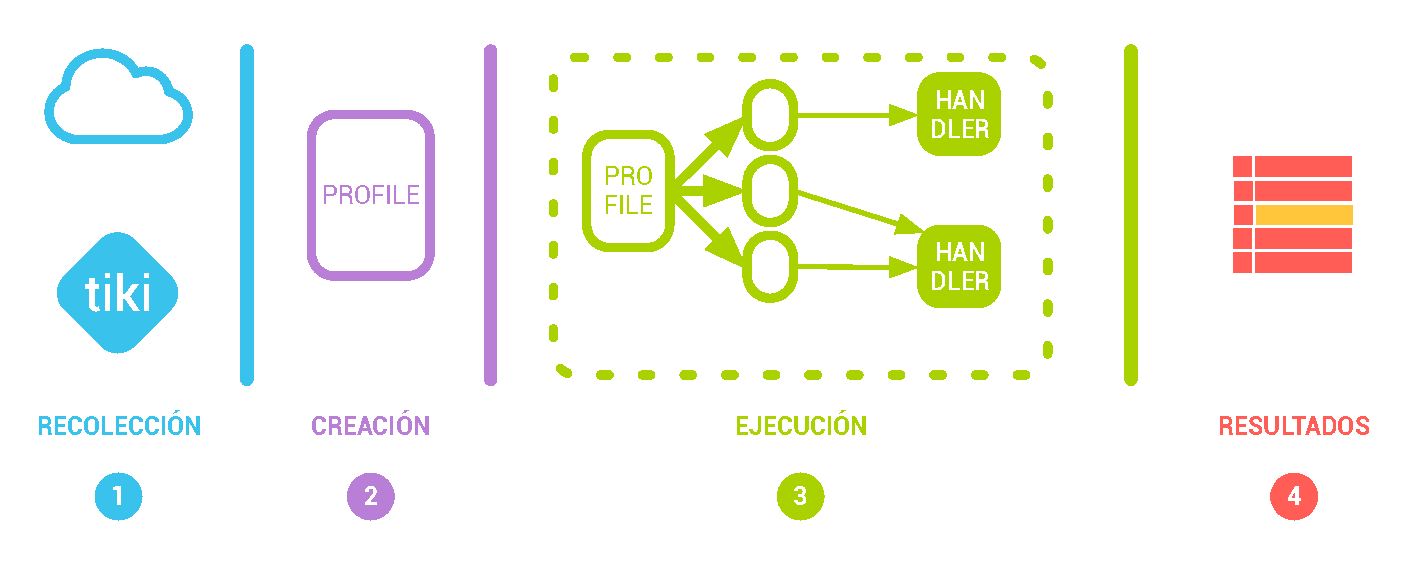
\includegraphics[width=\linewidth]{../graphics/fig_flujo_trabajo_profiles.eps}
\caption{}\label{fig:flujo_trabajo_profiles}
\end{figure}

\subsection{Recolección}

Una vez que hemos decidido trabajar con los \profiles{}, y sobre todo para esta primera estapa, debemos efectuarnos la siguiente pregunta: \q{¿Obtenemos un \profile{} que ya esté hecho o lo creamos desde cero?} 
Dependiendo de la respuesta, el flujo de trabajo puede variar ligeramente: si descargamos un \profile{} prefabricado hay que conseguirlo de algún lado mientras que, si lo creamos desde cero, no habría que hacer nada más (nos tendríamos que poner a escribir lo que deseamos crear, pero, sin depender de nada ni de nadie).

Para obtener un \profile{} que ya está diseñado de antemano, \tiki{} utiliza el concepto de \textit{repositorios}\footnote{El concepto de repositorio en \tiki{} se asemeja bastante, en idea, a los gestores de paquetes que se utilizan en varias distribuciones de Linux como: \texttt{apt} \cite{web:apt-debian}, \texttt{pacman} \cite{web:pacman-arch} o \texttt{yum} \cite{web:yum-fedora}.}. ¿Y qué son? Entendemos por repositorio aquel sitio centralizado donde se almacena y se mantiene un conjunto de \profiles{}. Se pueden clasificar en dos tipos:

\begin{itemize}
    \item \textbf{Externos}: Son en los que en nuestra instalación de \tiki{}, ésta necesita conectarse a un servidor externo para obtener un listado de todos los \profiles{} existentes. Por defecto, cuando instalamos \tiki{} por primera vez, nos añade el repositorio principal de \profiles{}: \url{http://profiles.tiki.org}. En dicho repositorio podemos encontrar todo tipo de \profiles{}, y éstos se pueden encontrar clasificados por funcionalidad, por número de versión, por la cantidad de votos que han recibido de otros usuarios que los han usado\ldots{} Pero también podemos optar por crear nuestro propio repositorio de \profiles{}, ya que, en el fondo son simplemente páginas \textit{wikis}.

    \item \textbf{Locales}: Son aquellos que se encuentran de manera local en nuestra plataforma y, por lo tanto, nuestra instalación de \tiki{} no necesita realizar ninguna petición a Internet. A su vez, se clasifican en dos formas: los que almacenan los \profiles{} en la misma instalación de \tiki{}, por ejemplo: \alma{} utiliza esta configuración\footnote{En la \sectionref{profile-creado-desde-cero} veremos que la ejecución de los \profiles{} de esta manera requieren un tratamiento especial, utilizan un componente añadido llamado \textit{Data Channel}.}; o replicar a su vez, una instalación de \tiki{} dedicada a \profiles{} (similar al repositorio oficial) pero en el que no hay un acceso a Internet. Por ejemplo: podría usarlo una empresa en una \textit{intranet} y separar así la instalación de trabajo de la del repositorio.
\end{itemize}

\subsection{Creación}

En esta segunda etapa, según la elección que hayamos tomado en la anterior, puede variar en la forma de llevarla a cabo: si decidimos obtener un \profile{} de algún repositorio es bastante probable que queramos ejecutarlo sin modificar nada de éste (aunque tenemos la opción de poder hacerlo); en cambio, si, por el contrario, hemos decidido crear un \profile{} desde el principio es, en esta etapa, en la que tenemos que pensar de manera creativa que queremos realizar con el mismo.

Cuando hablamos de un \profile{}, en concreto, nos estamos refiriendo al texto que encontramos dentro de una página \textit{wiki} y que es el que posee la información para que pueda ser evaluado por el intérprete de \profiles{} y que ejecute una acción (o varias) dentro de \tiki{}. Para poder crear uno hay que seguir unas reglas definidas: 

\begin{itemize}
    \item Utilizan un formato de marcado ligero llamado \yaml{}\footnote{Instamos al lector que si desconoce que es \yaml{} visite el \appendixref{yaml} para obtener unas nociones básicas, puesto que, los \profiles{} se basan en dicho formato y es necesario conocerlo para poder trabajar con ellos.} y, por lo tanto, el documento debe de estar conforme a esa especificación. Si no es así, el intérprete de \profiles{} lanzará un error informando al usuario de que no se ha podido leer correctamente el contenido del documento.

    \item Además, también tienen que ser escritos conforme a las reglas que dictaminen los \textit{Handlers} (los encargados de traducir la sintaxis \yaml{} en acciones concretas de \tiki{}, veremos más información en la \sectionref{ejecucion-profiles}).

\item Ya que los \profiles{} se almacenan en páginas \textit{wikis}, éstos pueden utilizar la potencia de la sintaxis \textit{wiki} y, por ejemplo: se puede dividir un \profile{} en múltiples partes y en cada una de ellas ir explicando su funcionamiento. O también, cada división puede ser un \profile{} que realice una tarea determinada. Lo importante es que cada bloque que pertenezca a un \profile{} debe de comenzar con \texttt{\{CODE(caption=>YAML)\}} y finalizar con \texttt{\{CODE\}}. A continuación, un ejemplo real que ilustra mejor los conceptos explicados:
\end{itemize}

\begin{figure}
\begin{pyglist}[language=text]
  Esto es un documento Wiki en el que ahora mismo utilizamos 
  la sintaxis wiki. A continuación en la siguiente linea 
  tenemos un bloque que marca el comienzo de un Profile.

  {CODE(caption=>YAML)}
  preferences: 
    feature_articles: y
  objects:
   -
    type: article_type
    ref: type
    data:
      name: New Type
      allow: [ ratings, comments ]
      show: [ author, reads, language ]
   -
    type: topic
    ref: topic
    data:
      name: New Topic
  {CODE}

  Podemos continuar editando nuestro documento con formato wiki 
  y cuando queramos, volvemos con un Profile que haga otra cosa
  (o que continúe con el anterior Profile).

  {CODE(caption=>YAML)}
  preferences: 
   feature_galleries: y
   feature_wiki: y
  {CODE}
\end{pyglist}
\caption{Ejemplo de una posible página \textit{wiki} con dos bloques de \profiles{}. Cada bloque puede realizar una tarea distinta o bien ser la misma tarea dividida en secciones y explicada por partes. Ejemplo extraído de: \url{http://profiles.tiki.org/Article+Handler}.}
\end{figure}

\subsection{Ejecución}
\label{section:ejecucion-profiles}

En las anteriores etapas se requería tomar ciertas decisiones que condicionaban, un poco, la manera de hacer las cosas frente a la creación de un \profile{}. En esta etapa, en cambio, no requiere ninguna interacción por parte del usuario ya que se realiza de forma automática cuando se ejecuta un \profile{}. Más bien nos sirve como excusa para presentar un concepto muy importante denominado: \textit{Handler}.

Un \textit{Handler} es un componente programado en la librería de \profiles{} que se encarga de leer y traducir a acciones reales (por ejemplo: crear una categoría, activar un recurso, asignar permisos\ldots{}) los bloques de texto que contengan sentencias de \profiles{} en una página \textit{wiki}. Actualmente hay dieciocho \textit{Handlers} cada uno encargado de realizar una tarea determinada, a saber:

\begin{itemize}
\item \textit{Article Handler}

\item \textit{Blog Handler}

\item \textit{Category Handler}

\item \textit{External Wiki Handler}

\item \textit{File Gallery Handler}

\item \textit{Forum Handler}

\item \textit{Menu Handler}

\item \textit{Module Handler}

\item \textit{Perspective Handler}

\item \textit{Plugin Alias Handler}

\item \textit{RSS Handler}

\item \textit{Template Handler}

\item \textit{Tracker Handler}

\item \textit{Transition Handler}

\item \textit{Webmail Handler}

\item \textit{Webservice Handler}

\item \textit{Wiki Handler}

\item \textit{Users Handler}
\end{itemize}

Cada uno tiene su propia sintaxis que se debemos respetar para que el intérprete de \profiles{} sea capaz de dar por bueno un \profile{} que hayamos escrito. Podemos encontrar toda la documentación referente a todas las posibles opciones que podemos poner visitando la documentación oficial \cite{web:handlers}. En la \figureref{ejemplo_opciones_handler_usuario}, se muestra las opciones que posee el \textit{Handler} de Usuarios (\textit{Users Handler}) y que podríamos utilizar para crear un \profile{} que implique la creación, de manera automatizada, de usuarios. Cabe añadir que la sintáxis no hace falta aprenderla de memoria, cuando tengamos alguna necesidad, simplemente hay que visitar la web y consultar lo que deseemos.

\begin{figure}
\centering
\includegraphics[width=\linewidth]{../graphics/fig_ejemplo_opciones_handler_usuario.png}
\caption{Estas son las opciones que se pueden poner en un \profile{} si queremos crear un usuario.}\label{fig:ejemplo_opciones_handler_usuario}
\end{figure}

\subsection{Resultados}

En esta etapa, la última, lo que obtenemos son los resultados de manera visible de lo que hayamos realizado con nuestro \profile{}. Ya sean cambios muy drásticos o, por contra, muy leves. A partir de aquí podemos repetir el flujo de trabajo con los \profiles{} desde el principio y tantas veces como deseemos, solo que en las siguientes veces, ya no tendremos que diseñarlo, pues, éste fue creado anteriormente.

\section{Explicación de la interfaz de los Profiles}

La administración de los \profiles{} por parte de un administrador es bastante simple y, prácticamente, no requiere de aprendizaje alguno. Si un usuario visita la siguiente dirección: \url{http://localhost/tiki-admin.php?page=profiles} lo que se encontrará es lo que se muestra en la \figureref{admin_profiles_pestaña_1} (un panel principal dividido en tres pestañas):

\begin{itemize}
    \item \textit{Ejecutar \profiles{} (Apply \profiles{})}: Mostrada en la figura anterior, esa pestaña es la encargada de listar todos los \profiles{} que ha encontrado \tiki{} en un determinado repositorio (sea el oficial o cualquier otro). Desde aquí el usuario puede elegir y filtrar, según preferencias, que tipos de \profiles{} desea ver. Tiene la opción de obtener más información acerca de lo que hace un \profile{} en concreto (que cosas crea y que cambia) y, por supuesto, de ejecutarlo en su instalción de \tiki{} (\figureref{ejecucion_profile}).

\item \textit{Exportar}: Esta pestaña permite al administrador volcar todos los datos de configuración que haya realizado sobre \tiki{}. Pero, ojo, ¡sólo las preferencias! Si se ha ejecutado anteriormente un \profile{} que genera grupos, por poner un ejemplo, no se guarda ni los grupos creados ni la información que contengan éstos (\figureref{exportar_configuracion_pestaña_2}).

\item \textit{Avanzado}: Aquí se pueden añadir nuevos repositorios, crear múltiples \textit{Data Channels} (como se dijo antes, entenderemos el concepto con un ejemplo práctico en la siguiente sección) y, en última instancia, existe un apartado para ejecutar los \profiles{} directamente. Esto nos sirve para probar configuraciones útiles o para realizar ejecuciones de prueba. Hay que tener especial cuidado porque como se indica en la imagen, se pueden hacer cambios irreversibles en la configuración de la base de datos (\figureref{pestaña_avanzado_3}).
\end{itemize}

\begin{figure}
\centering
\includegraphics[width=\linewidth]{../graphics/fig_admin_profiles_pestaña_1.png}
\caption{Panel principal de administración de los \profiles{}.}
\label{fig:admin_profiles_pestaña_1}
\end{figure}

\begin{figure}
\centering
\includegraphics[width=\linewidth]{../graphics/fig_ejecucion_profile.png}
\caption{Panel donde podemos listar los \profiles{} que tiene un repositorio y ejecutarlos.}\label{fig:ejecucion_profile}
\end{figure}

\begin{figure}
\centering
\includegraphics[width=\linewidth]{../graphics/fig_exportar_configuracion_pestaña_2.png}
\caption{Panel donde podemos exportar las preferencias que hayamos modificado de \tiki{}. Se puede utilizar como método de copia de seguridad para restaurar posteriormente la misma configuración.}\label{fig:exportar_configuracion_pestaña_2}
\end{figure}

\begin{figure}[H]
\centering
\includegraphics[width=\linewidth]{../graphics/fig_pestaña_avanzado_3.png}
\caption{Panel que nos permite añadir nuevos repositorios, agregar nuevos \textit{Data Channels} y ejecutar \profiles{} de prueba.}\label{fig:pestaña_avanzado_3}
\end{figure}

\section{Un ejemplo con Profiles}

Vamos a mostrar dos ejemplos: uno sencillo y otro más complejo para entender mejor todos los conceptos que han sido presentados hasta ahora. En ambos casos, se pretende explicar al lector los pasos necesarios que tiene que seguir un hipotético administrador que desea crear, todo de manera automatizada, una página \textit{wiki} denominada \q{Prueba}, una categoría (también con el mismo nombre) en cuyo interior se encuentra la página anterior y, por último, cambiar el tema visual que utiliza \tiki{} (por defecto en azul) por otro en amarillo. La diferencia principal de los dos ejemplos estriba en la forma de llevarlo a cabo, en el primero, se asume que hay un \profile{} en el repositorio oficial. En el segundo, en cambio, se crea el \profile{} desde cero y se ejecuta en la instalación local utilizando para ello los \textit{Data Channels}.

\subsection{Profile ejecutado desde un repositorio}

Este es el caso más sencillo, los pasos son los siguientes:

\begin{enumerate}
\item Como administradores nos dirigimos a la página de administración de \profiles{} (recordemos: \url{http://localhost/tiki-admin.php?page=profiles}).

\item Listamos los \profiles{} existentes en el repositorio oficial y buscamos uno que se llama \texttt{Test\_Wiki\_Group} (podemos basarnos en las imágenes de la anterior sección puesto que este paso no cambia prácticamente nada, sólo el nombre del \profile{} a listar, \figureref{ejecucion_profile}).

\item Rellenamos las casillas con los nombres apropiados, el nombre de la página \textit{wiki}, el de la categoría y el del grupo y pulsamos ejecutar.

\item \textit{¡Et voilá!} Acción ejecutada, podemos comprobar en la \figureref{profile_ejemplo} que se cumple lo que el \profile{} prometía.

\end{enumerate}

\begin{figure}
\centering
\includegraphics{../graphics/fig_profile_ejemplo.png}
\caption{Categoría creada con una página wiki tal y como el Profile había especificado.}\label{fig:profile_ejemplo}
\end{figure}

\subsection{Profile ejecutado desde una instalación local}
\label{section:profile-creado-desde-cero}

En este caso, un poco más complejo, el \profile{} se ejecuta en una instalación local por lo que los pasos varían en varios puntos respecto al anterior ejemplo:

\begin{enumerate}

    \item Dado que en esta situación tenemos que crear el \profile{} desde cero, conviene pensar (como ya hicimos anteriormente) en términos absolutos: ¿qué queremos conseguir? y ¿cómo lo vamos a realizar? La respuesta a la primera pregunta está clara, lo definimos anteriormente: crear una página \textit{wiki} con un nombre determinado, una categoría de idéntico nombre que agrupe al anterior recurso y cambiar el color del tema visual. La respuesta para la segunda pregunta nos obliga a pensar en términos de \textit{Handlers}, en este caso, ¿qué \textit{Handlers} intervienen? Para crear la página \textit{wiki} es casi seguro que necesitaremos el \textit{Wiki Handler}, para la categoría utilizaremos el \textit{Category Handler} y para cambiar el color al ser una preferencia se puede poner directamente en el \profile{} (en la \figureref{listado_profile_ejemplo} tenemos de manera completa el \profile{} que utilizaremos, dejamos al lector la tarea de investigar y comprender las opciones que se listan utilizando para ello la bibliografía existente).

\item Una vez que tenemos claro como va a ser el \profile{}, hay que crear una página \textit{wiki} para almacenarlo, denominaremos a la página \textit{wiki} \texttt{primer\_profile} (no hay que olvidar este nombre ya que lo utilizaremos después y lo debemos respetar tal y como está escrito), copiamos el \profile{} (\figureref{listado_profile_ejemplo}), añadimos los fragmentos al principio (\texttt{\{CODE(caption=>YAML)\}}) y al final (\texttt{\{CODE\}}) del \profile{} y guardamos la página (\figureref{editar_primer_profile}).

\item Ya hemos creado la página \textit{wiki} con nombre \texttt{primer\_profile} y el \profile{} dentro. A partir de ahora podemos modificar la página tantas veces como queramos y recuperar su contenido con el historial de versiones.

\item Debido a que el \profile{} se va a ejecutar de manera local tenemos que utilizar los \textit{Data Channels} que es el encargado de avisar a \tiki{} para que no busque en otro repositorio externo, sino dentro de si mismo\footnote{Aunque los \textit{Data Channels} tienen más usos que el que se lista en este ejemplo. Si queremos ver todos y aprender más sobre ellos conviene visitar su página \textit{wiki} \cite{web:data-channels}.}. Para ello vamos a la pestaña de Avanzado en el panel de administración de \profiles{} (\figureref{pestaña_avanzado_3}) y tenemos que introducir lo siguiente en la casilla de \textit{Data Channels}:

\begin{pyglist}[language=text]
  mi_prueba, tiki://local, primer_profile, Admins
\end{pyglist}
 
La documentación de los \textit{Data Channels} explican el significado de cada elemento, un resumen:
\begin{itemize}
\item \textit{mi\_prueba}: Tenemos que denominar al \textit{Data Channel} con un identificador único, puede ser cualquier nombre que sea un carácter alfanumérico incluyendo también al símbolo \_.

\item \textit{tiki://local}: Indica a \tiki{} que utilice la página \textit{wiki} como \profile{} ya que está en su propia base de datos y no en un repositorio externo.

\item \textit{primer\_profile}: Indicamos a \tiki{} cual es la página en concreto que se usará como \profile{}. Se corresponde con el nombre que dimos a la página \textit{wiki} anteriormente.

\item \textit{Admins}: Especificamos que grupo tiene derecho a ejecutar el \profile{}. Se recomienda poner grupos que sean de confianza (es una imprudencia asignar el \profile{} a un grupo como \texttt{Anonymous} donde cualquiera puede ejecutarlo). Si queremos poner más grupos, se pueden poner separados por coma, por ejemplo: \texttt{Admins, Grupo1, Grupo2}.
\end{itemize}

\item Guardamos la información que hemos escrito en el \textit{Data Channel}. ¡La parte más difícil ya está superada! Ahora tenemos que buscar la manera de poder ejecutar el \profile{}, y para ello vamos a crear una interfaz gráfica con un botón al que siempre podamos acudir cuando queramos utilizar el \profile{} (en la \figureref{interfaz_plugin_data_channel} vemos un ejemplo de como quedaría al final del proceso). Para ello vamos a generar una nueva página \textit{wiki} denominada \texttt{mi\_profile\_interfaz} y copiaremos el contenido de la \figureref{datachannel} (en la descripción del mismo se explica el significado de todo el código).

\item ¡Y ya está! Cada vez que queramos utilizar dicho \profile{} acudimos a la página \texttt{mi\_profile\_interfaz} pulsamos el botón y este ejecuta el \profile{} guardado en \texttt{primer\_profile}. Hay que avisar que si un usuario que no pertenezca al grupo \texttt{Admins} (que así fue como lo especificamos en la linea de los \textit{Data Channel} en el paso 4) intenta ejecutar el \profile{}, éste no hará nada. No obstante un usuario que no esté autorizado a ejecutar \profiles{} no debería ver tampoco esta página así como donde está el \profile{} en sí (nos evitaremos muchos problemas a la larga).
\end{enumerate}

\begin{figure}
\begin{pyglist}[language=text]
  {CODE(caption=>YAML)}
  preferences: 
   style_option: kiwi.css
   enable: [ feature_wiki ]
  objects:
   -
    type: wiki_page
    data:
      name: Prueba
      content: Creando una wiki con profiles
      ref: pagina_prueba
   -
   type: category
    data:
     name: Prueba
     items:
      - [ wiki_page, pagina_prueba ]
  {CODE}
\end{pyglist}
\caption{En la sección de \code{preferences} se pueden poner las preferencias directamente que encontramos en la tabla \texttt{tiki\_preferences} como ya comentamos. Hay que añadir que al crear múltiples recursos en este \profile{} hacemos uso de las referencias (aquellas que comienzan con \texttt{ref}, lo usaremos más adelante \cite{web:object-references}).}
\label{fig:listado_profile_ejemplo}
\end{figure}

\begin{figure}
\begin{pyglist}[language=text]
  {DATACHANNEL(channel=mi_prueba)}{DATACHANNEL}
\end{pyglist}
\caption{Este código copiado tal cual en la página \textit{wiki} genera la interfaz gráfica e invoca al \profile{} que hemos creado antes. Hay que observar que en donde pone \texttt{channel} se ha escrito el nombre del \textit{identificador que dimos en el \textit{Data Channel}}. En la documentación oficial tenemos más información acerca del \texttt{Plugin Data Channel} que es como se denomina esta herramienta que genera interfaces para los \profiles{} \cite{web:plugin-code}.}
\label{fig:datachannel}
\end{figure}

\begin{figure}
\centering
\includegraphics{../graphics/fig_editar_primer_profile.png}
\caption{Escribimos el contenido del \profile{} en una página wiki.}\label{fig:editar_primer_profile}
\end{figure}

\begin{figure}
\centering
\includegraphics{../graphics/fig_interfaz_plugin_data_channel.png}
\caption{Interfaz gráfica generada por el \textit{plug-in} \textit{Data Channel}, podemos ejecutar el \profile{} cómodamente con un clic de ratón.}\label{fig:interfaz_plugin_data_channel}
\end{figure}

\section{Implementación interna de los Profiles}

A continuación, para todas aquellas personas que estén interesadas en desarrollar y/o mejorar un \textit{Handler} o simplemente desean saber más sobre como funciona internamente la plataforma, se dará una explicación de las partes más interesantes que hacen posible que los \profiles{} existan tal y como los conocemos. Para ello, se explicará como se desarrolló el \textit{Users Handler} (el que se encarga de crear usuarios) por ser éste bastante sencillo de entender y que fue creado por el autor del \pfc{}. Aconsejamos al lector leer (si no se ha realizado anteriormente) el \appendixref{apendice-c} para obtener primero una visión complementaria de como está estructurado el código de \tiki{}. Sin más dilaciones, comenzamos.

\subsection{¿Cómo funciona por dentro un Handler?}

El código fuente que da vida a los \profiles{} se halla en la carpeta \code{lib/profilelib}. Dentro de dicho directorio nos encontramos con cuatro archivos importantes:

\begin{itemize}
    \item \code{profilelib.php}: Esta librería es la que da el funcionamiento principal de todo el código y la encargada de interpretar los documentos en formato \yaml{}, de buscar referencias de objetos en el propio \profile{}, de devolver un mensaje de error al usuario si algo ha ido mal, y de realizar las peticiones a otras plataformas \textit{wiki} si el \profile{} está alojado en otros repositorios. Normalmente el código que hay aquí no hace falta tocarlo para poder crear un \textit{Handler} a no ser que queramos añadir una nueva forma de interpretar los documentos (por ejemplo: que en lugar de leerlos en formato \yaml{} los hiciese en formato \json{}).

\item \code{channellib.php}: Esta librería es la que lleva el manejo de los \textit{Data Channels}, algunas tareas que realiza es la comprobación de que un \textit{Data Channel} puede ser ejecutado por un usuario, y otra es cargar en la interfaz los Channels que hay guardados en la base de datos. De manera idéntica a lo que se dijo en el punto anterior, no debemos modificar nada de este fichero.

\item \code{listlib.php}: Esta librería es la encargada de realizar peticiones a otros servidores y generar una base de datos con los \profiles{} que hay existentes en dicho repositorio.

\item \code{installlib.php}: Esta librería es la encargada de crear los dieciocho \textit{Handlers} que hay actualmente. Hay una clase principal denominada \code{Tiki\_Profile\_InstallHandler} y es sobre la que deberemos heredar si queremos crear un nuevo \textit{Handler}. Dicha clase determina los siguientes métodos: \code{\_\_construct()}, \code{canInstall()}, \code{install()}, \code{replaceReferences()} y \code{\_install()} y son importantes puesto que las clases que implementemos tendrán que sobre-escribirlos (dependiendo de las necesidades del \textit{Handler}). El nombre de la clase utilizado para el \textit{User Handler} es \code{Tiki\_Profile\_InstallHandler\_User} y hereda de \code{Tiki\_Profile\_InstallHandler}, los métodos que implementa son los siguientes:
\begin{itemize}
\item \code{getData()}: Este método lo que realiza es obtener la información del \profile{} (todo lo que le corresponde al \textit{Handler} de usuarios) y reemplazar las referencias que haya.
\item \code{canInstall()}: Este método se encarga de preguntar si se puede instalar el \profile{} o no y para ello comprueba que hay algo escrito dentro del \profile{}.
\item \code{\_install()}: Este es el método más importante ya que es el que realiza el grueso de la operación de añadir usuarios. Lo que hace es comprobar si están los campos que necesita el \textit{Handler} para funcionar y si es así llama a la librería \code{userlib.php} que es la encargada de crear nuevos usuarios.
\end{itemize}
En la \figureref{user-handler-impl} se muestra la implementación completa (por ser bastante breve) del \textit{User Handler}.
\end{itemize}

\begin{figure}
\begin{pyglist}[language=php]
  <?php
  class Tiki_Profile_InstallHandler_User extends Tiki_Profile_InstallHandler
  {
    function getData()
    {
      if( $this->data )
        return $this->data;
      $data = $this->obj->getData();
      $this->replaceReferences($data);

      return $this->data = $data;
    }

    function canInstall()
    {
      $data = $this->getData();
		
      if (isset($data)) return true;
      else return false;
    }
	
    function _install()
    {
      if ($this->canInstall())
      {
        global $userlib; if (!$userlib) require_once 'lib/userslib.php';

        $user = $this->getData();
				
        if (!$userlib->user_exists($user['name'])) {
          $pass = isset($user['pass']) ? $user['pass'] : $user['name'];
          $email = isset($user['email']) ? $user['email'] : '';
          if (isset($user['change']) && $user['change'] === false) {
            $userlib->add_user($user['name'], $pass, $email);
          } else {
            $userlib->add_user($user['name'], $pass, $email, $pass, true);
          }
        }

        if (isset($user['groups'])) {
          foreach ($user['groups'] as $group) {
            $userlib->assign_user_to_group($user['name'], $group);
          }
        }
				
        return $userlib->get_user_id($user['name']);
       }
    }
  }
\end{pyglist}
\caption{Implementación del \code{Users Handler}.}
\label{fig:user-handler-impl}
\end{figure}
